\documentclass[final,hyperref={pdfpagelabels=true},t]{beamer} 
% language
\usepackage[english]{babel}

% setup fonts
%\usepackage{GillSans}
\usepackage[scaled=0.85]{helvet}
\usefonttheme{professionalfonts}
\usepackage[scaled=0.8]{beramono}
\usepackage{arev}
\usepackage{fix-cm}
\usepackage[T1]{fontenc}

% packages
\usepackage{varwidth}
\usepackage{algorithmic}
\usepackage{rotating}
\let\Tiny=\tiny
\usepackage[beamer,matrixmath,matrixshorts,vectorshorts,statisticsmath,genericmath,tkzberge]{dgleich}
\graphicspath{{./}{./figures/}{./code/}}
\usepackage{microtype}
\usepackage{textcase}
\usepackage{tabularx}
\usepackage[absolute,overlay]{textpos}
\usepackage[texcoord]{eso-pic}



% display agnostic commands

% use a fancysans 
% \newcommand{\fancysansfamily}{GillSans-TLF}
% \newcommand{\fancysans}{\usefont{T1}{GillSans-TLF}{m}{n}}
% \newcommand{\fancysanstext}[1]{{\fancysans #1}}
% \newcommand{\fancysanstextit}[1]{{\usefont{T1}{GillSans-TLF}{m}{it} #1}}

% use Helvetica
\newcommand{\fancysansfamily}{phv}
\newcommand{\fancysans}{\usefont{T1}{phv}{m}{n}}
\newcommand{\fancysanstext}[1]{{\fancysans #1}}
\newcommand{\fancysanstextit}[1]{{\usefont{T1}{GillSans-TLF}{m}{it} #1}}

% define a command for fancy text fractions if the font supports it
\newcommand{\textfrac}[1]{#1}

% change the margins
\newenvironment{changemargin}[2]{%
\begin{list}{}{%
\setlength{\topsep}{0pt}%
\setlength{\leftmargin}{#1}%
\setlength{\rightmargin}{#2}%
\setlength{\listparindent}{\parindent}%
\setlength{\itemindent}{\parindent}%
\setlength{\parsep}{\parskip}%
}%
\item[]}{\end{list}}

%adjust the TPHorizModule and TPHorizModule units to the displayed mm %grid
%\TPGrid[0mm,0mm]{100}{100}

%puts a graphic at the absolute position described by the grid
%#1 x, #2 y, #3 , #4 graphic
\newcommand\putpic[4][]{%
        \begin{textblock}{0}(#2,#3)%
  \begin{picture}(0,0)(0,0)\includegraphics[#1]{#4}\end{picture}%
     \end{textblock}%
} 
\newcommand{\putat}[3]{%
\begin{textblock}{0}(#1,#2)%
\begin{picture}(0,0)(0,0){#3}\end{picture}%
\end{textblock}}%




%%
%% SETUP the slide appearance
%% These commands are often nasty, we begin by defining a set of colors
%% then the next include actually specifies all the beamer layout commands.
%%

% Colors
\definecolor{accentlight}     {RGB}{31,73,125}
\definecolor{accentheavy}      {RGB}{153,0,0}
\definecolor{shadelight}{RGB}{142,180,227} % light blue
%\definecolor{shadeheavy}{RGB}{203,203,203}
\definecolor{shadeheavy}{RGB}{196,189,151}
\colorlet{shadelight}{shadeheavy!50!white}
\definecolor{backgroundaccent}{RGB}{196,189,151}
\definecolor{background}{RGB}{238,236,225}
\definecolor{neutralshade}{gray}{0.85}  

% derived colors
\colorlet{shadecolor}{neutralshade}
\colorlet{lighttextcolor}{shadecolor!50!black}
\colorlet{boxshade}{backgroundaccent}
\colorlet{boxframe}{backgroundaccent}

\usetheme{GleichPosterPaloAlto}

% setup Poster
\usepackage[orientation=landscape,size=a0,scale=1.1]{beamerposter}       

% setup pieces on top of the poster.


% Poster columns
% fix spacing in the columns
\makeatletter
\newcommand{\defaultmetrics}{%
% Setup parskip (just ripped from parskip.sty)
\parskip=0.5\baselineskip \advance\parskip by 0pt plus 2pt%
\parindent=\z@%
\def\@listI{\leftmargin\leftmargini%
   \partopsep\z@% added by G. Partosch
   \topsep\z@ \parsep\parskip \itemsep\z@}%
\let\@listi\@listI%
\@listi%
\def\@listii{\leftmargin\leftmarginii%
   \labelwidth\leftmarginii\advance\labelwidth-\labelsep%
   \partopsep\z@% added by G. Partosch
   \topsep\z@ \parsep\parskip \itemsep\z@}%
\def\@listiii{\leftmargin\leftmarginiii%
    \labelwidth\leftmarginiii\advance\labelwidth-\labelsep%
    \partopsep\z@% added by G. Partosch
    \topsep\z@ \parsep\parskip \itemsep\z@}%
\justifying% Make everything Justified    
}
\newcommand{\postercolumn}[2][t]{%
  \column[#1]{#2}%
  \normalsize\defaultmetrics\ignorespaces%
}
\makeatother


%% 
%% Display specific commands.  
%%

\newcommand{\reftext}[1]{\fancysanstextit{\textcolor{accentlight}{#1}}}

\newcommand{\noterlap}[1]{\rlap{\color{lighttextcolor}#1}}

\newcommand{\plotbox}[1]{%
  \setlength\fboxrule{1pt}\fcolorbox{boxframe}{boxshade}{#1}%
}  
\newcommand{\cplotbox}[1]{%
  \begin{center}\setlength\fboxrule{1pt}\fcolorbox{boxframe}{boxshade}{#1}\end{center}%
}  
\newcommand{\mathbox}[2][0.8]{%
  \begin{center}%
    \setlength\fboxrule{1pt}\fcolorbox{boxframe}{boxshade}{%
    \begin{beamercolorbox}[sep=1em,wd=#1\linewidth]{mybox}%
    #2%
    \end{beamercolorbox}%
    }%
  \end{center}%
}

\newcommand{\deemph}[1]{%
  {\itshape\color{lighttextcolor}%
  #1%
 }
}

\newcommand{\captext}[1]{%
 {\scriptsize\deemph{#1}}%
}


\newenvironment{highlight}[1][1ex]{%
  \begin{list}{}{%
    \setlength{\topsep}{1ex}%
    \setlength{\itemsep}{1ex}%
    %\setlength{\parsep}{2pt}%
    \setlength{\listparindent}{0pt}%
    \setlength{\itemindent}{0pt}%
    \setlength{\leftmargin}{1ex}%
    \setlength{\rightmargin}{0pt}%
  }\color{accentlight}\item%
}{%  
  \end{list}%
}


\usetikzlibrary{fit,shapes}
\usepackage{calc}
\usepackage{wrapfig}
\usepackage{microtype}
\usepackage{paralist}
\usepackage{epstopdf}

%% Poster specific macros
\DeclareMathOperator{\maxvol}{MaxVol}
\DeclareMathOperator{\vol}{Vol}
\DeclareMathOperator{\totalvol}{TotalVol}
\DeclareMathOperator{\swaps}{Swaps}
\DeclareMathOperator{\cut}{Cut}
\newcommand{\coll}{\mathcal{C}}
\newcommand{\map}{\tau}
\newcommand{\algo}[1]{\MakeTextLowercase{\textsc{#1}}}
\renewcommand{\emph}[1]{\textcolor{accentlight}{#1}}

\newcommand{\Xsequence}{X_{0}, \dots, X_{T} }
\newcommand{\Ysequence}{Y_{0}, \dots, Y_{T} }

%\usepackage{epstopdf}
%\setgraphicspath{{./}{./figures/}}

%% Title page
\title[Fancy Posters]{%
  OVERLAPPING CLUSTERS FOR DISTRIBUTED COMPUTATION
}

%% Normal authors
\author[Please email David Gleich (dgleich@purdue.edu) for questions]{%%
Reid ANDERSEN - Microsoft
David GLEICH - Purdue \and
Vahab MIRROKNI - Google}

%% Stylized authors, just copy and update
\renewcommand{\fancyauthor}{%
			\fancysans 
      {\large REID} {\large ANDERSEN} 
        {\small $\cdot$ MICROSOFT CORPORATION} {\Large\strut}\par%
      {\large DAVID F.} {\large GLEICH} 
        {\small $\cdot$ PURDUE UNIVERSITY} {\Large\strut}\par%
      {\large VAHAB S.} {\large MIRROKNI} 
        {\small $\cdot$ GOOGLE RESEARCH $\cdot$ NYC} {\Large\strut}\par%
}        

%% Presentation Venue and date
\date{WSDM2012 - February 2012}

%% Add link to code
\renewcommand{\footlinecomment}{\bfseries 
Our code is available online: Google ``overlapping gleich'' to find it.}


\begin{document}


\defaultmetrics
%% A beamerposter only has a single frame
\begin{frame}
\vspace{0.5\pageborder}

\begin{columns}

%% Adjust 0.35 for the width of the first column
\postercolumn{0.35\textwidth}
\begin{block}{1. The idea}
\RaggedRight

%% Here is a ``wrapfig'' like setup.
\begin{tabularx}{\linewidth}{U@{\quad}l}
Scalable, distributed algorithms must address
communication.  We investigate
\emph{overlapping clusters} -- see figure -- 
for graph computations. This setup 
stores more of the graph than required but 
affords the ease of implementation
of vertex partitioned algorithms. 
\begin{highlight}
 Carefully using overlap allows us
to reduce communication in distributed graphs
computations (on some graphs).
\end{highlight}
&
\fcolorbox{neutralshade}{neutralshade}{
\raisebox{1ex-\height}{
\vspace{1em}

\hspace{0.25em}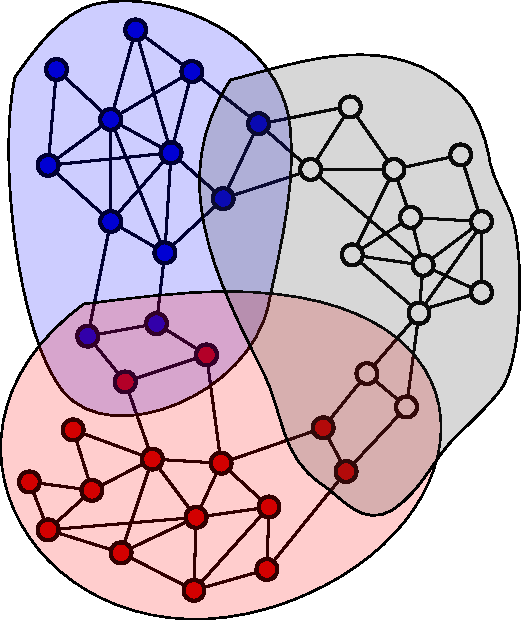
\includegraphics[width=6.5cm]{overlapping-figure}\hspace{0.25em}

\vspace{1em}
}
}

\end{tabularx}

\end{block}


%% Start of the second column
\begin{block}{2. Related work}
\RaggedRight

The motivation above draws on recent work in
\emph{communication avoiding} algorithms.  Mohiyuddin 
et al. (SC09) design a matrix-powers kernel that gives rise to
an overlapping partition.  Fritzsche et al. (CSC2009) develop
an overlapping clustering for a Schwarz method.  \emph{Both techniques
extend an initial partitioning with overlap.  Our procedures
generates overlap directly.}  Indeed, Schwarz methods are commonly
used to capitalize on overlap.

Elsewhere, overlapping communities (Ahn et al, Nature 2009; 
Mishra et al. WAW2007) are now a popular model of 
structure in social networks.  These have long 
been studied in statistics (Cole and Wishart, CompJ 1970).


\end{block}

 
\vspace{0.5\pageborder} 
\begin{block}{3. Problem setup}
\RaggedRight

{{\large \fancysanstext{\textls[150]{NOTATION}}}}
Let \alert{$\vol(C)$} $ = $ sum of degrees for vertices in cluster $C$.

\begin{highlight}
Given a graph $G$, an \alert{overlapping 
clustering $(\mathcal{C},\tau)$} is a set
of clusters $\mathcal{C}$ and a mapping from each vertex 
to a home cluster $\tau$.  The total number of edges in a
cluster ($\vol(C)$) is constrained by \alert{$\maxvol$}.  
\end{highlight}

In a random walk on an
overlapping clustering, the walk moves from cluster to
cluster.  On leaving a cluster, it goes to the
home cluster of the new vertex: e.g.
\begin{tikzpicture}[x=1.5cm,y=1.5cm,baseline=(a.south)]
  \GraphInit[vstyle=Hasse]
  \renewcommand{\VertexLineWidth}{2pt}
  \renewcommand{\EdgeLineWidth}{2pt}
  \renewcommand{\VertexLightFillColor}{accentlight}
  \Vertex[x=0,y=0]{a}
  \Vertex[x=1,y=0]{b}
  \renewcommand{\VertexLightFillColor}{DarkGreen}
  \Vertex[x=2,y=0]{c}
  \node[draw,fill=accentlight,fill opacity=0.3,thick,rounded rectangle,fit=(a) (b) (c),inner sep=6pt] {};
  \renewcommand{\VertexLightFillColor}{accentheavy}
  \Vertex[x=3,y=0]{d}
  \Vertex[x=4,y=0]{e}
  \node[draw,fill=accentheavy,fill opacity=0.3,thick,rounded rectangle,fit=(d) (e),inner sep=6pt] {};
  \tikzset{EdgeStyle/.style={->}}
  \renewcommand{\EdgeColor}{gray}
  \Edge(a)(b)
  \Edge(b)(c)
  \renewcommand{\EdgeColor}{black}
  \Edge(c)(d)
  \renewcommand{\EdgeColor}{gray}
  \Edge(d)(e)
  %\node[x=2.5,y=-1] {Swap};
  %\draw (2.5,-1) node {Swap};
\end{tikzpicture}
In this illustration, the color indicates
the home vertices for a cluster.  (See the example
above too.)
\emph{A transition between clusters is a swap, and requires a 
communication if the underlying graph is distributed by 
clusters}.  
We thus wish to minimize
swaps in a random walk.  Let $\rho_T(v) = $
the expected fraction of steps that swap in a $T$-step 
walk starting from $v$.  We study:
\alert{$\rho_\infty = \lim_{T \to \infty} \frac{1}{n} \sum_{v} \rho_T(v)$},
the fraction of steps with swaps for a long walk.
\emph{For a cycle graph, we can prove that overlap reduces
the communication.}



%\begin{center}
%\fcolorbox{neutralshade}{neutralshade}{
%\begin{beamercolorbox}[sep=0.25em,wd=0.6\linewidth]{mybox}
% \[ \begin{array}{cl}
%     \text{maximize} & \alpha \vw^T \vx + \frac{\beta}{2}\sum Y_{ii',jj'}\\
%     \text{subject to}& \mA \vx \le \ve, Y_{ii',jj'} \le x_{i,i'}, Y_{ii',jj'} \le x_{j,j'} \\
%                      & x_{i,i'} \in \{0,1\}.
%   \end{array} \]
%\end{beamercolorbox}
%}
%\end{center}

{{\large \fancysanstext{\textls[150]{THEOREM}}}
Consider a large cycle $C_n$ of $n=M\ell$ nodes for a large
number $M>0$, 
and let the maximum volume of a cluster $\maxvol$ be  $2\ell$. 
Let $P$ be the optimal partitioning of $G$ to non-overlapping clusters of size at most
$\maxvol$ and $\rho_\infty^*$ be the swapping probability of $P$.  
There exists an overlapping cover with $\totalvol$ of 2$\vol(G)$ whose 
swapping probability $\rho_\infty'$  is less than $\rho_\infty^*/\Omega(\maxvol)$. 
}

(Proof Sketch) The overlapping clustering that achieves this bound is:
 \fcolorbox{neutralshade}{neutralshade}{%
   \begin{beamercolorbox}[sep=0.15em,wd=\linewidth]{mybox}
     \centering
      \begin{tikzpicture}[x=1.5cm,y=1.5cm]
  \GraphInit[vstyle=Hasse]
  \renewcommand{\VertexLineWidth}{1pt}
  %\SetGraphUnit{0.5}
  %\draw[help lines] (0,0) grid (16,2);
  \fill[color=background] (-0.5,-1.5) rectangle (15.5,1.5);
  %\fill[color=accentheavy] (-4.5,-0.5) rectangle (3.5,0.5);
  %\fill[color=accentlight] (-0.5,-0.5) rectangle (7.5,0.5);
  %\fill[color=backgroundaccent] (-0.5,-0.5) rectangle (7.5,0.5);
  \Vertex[x=-5,y=0,empty]{L}
  \renewcommand{\VertexLightFillColor}{DarkGreen}
  \Vertex[x=-4,y=0,Lpos=90]{13}
  \Vertex[x=-3,y=0,Lpos=90]{14}
  \renewcommand{\VertexLightFillColor}{accentheavy}
  \Vertex[x=-2,y=0,Lpos=90]{15}
  \Vertex[x=-1,y=0,Lpos=90]{16}
  %\Vertices[x=-4,y=0,Lpos=90]{line}{13,14,15,16}
  \draw (-2.5,-1) node {Cycle wrap};
  \Edges(L,13,14,15,16) 
  %\Vertices[Lpos=90]{line}{1,2,3,4,5,6,7,8}
  \Vertex[x=0,y=0,Lpos=90]{1}
  \Vertex[x=1,y=0,Lpos=90]{2}
  \renewcommand{\VertexLightFillColor}{accentlight}
  \Vertex[x=2,y=0,Lpos=90]{3}
  \Vertex[x=3,y=0,Lpos=90]{4}
  \node[draw,inner sep=6pt,fill=accentheavy,fill opacity=0.3,thick,rounded rectangle,fit=(13) (14) (15) (16) (1) (2) (3) (4)] {};
  \Edges(16,1,2,3,4) 
  \Vertex[x=4,y=0,Lpos=90]{5}
  \Vertex[x=5,y=0,Lpos=90]{6}
  \renewcommand{\VertexLightFillColor}{backgroundaccent}
  \Vertex[x=6,y=0,Lpos=90]{7}
  \Vertex[x=7,y=0,Lpos=90]{8}
  \Edges(4,5,6,7,8) 
  \node[draw,inner sep=12pt,fill=accentlight,fill opacity=0.3,thick,rounded rectangle,fit=(1) (2) (3) (4) (5) (6) (7) (8)] {};
  \Vertex[x=8,y=0,Lpos=90]{9}
  \Vertex[x=9,y=0,Lpos=90]{10}
  \renewcommand{\VertexLightFillColor}{DarkGreen}
  \Vertex[x=10,y=0,Lpos=90]{11}
  \Vertex[x=11,y=0,Lpos=90]{12}
  \Edges(8,9,10,11,12) 
  \node[draw,inner sep=6pt,fill=backgroundaccent,fill opacity=0.3,thick,rounded rectangle,fit=(5) (6) (7) (8) (9) (10) (11) (12)] {};
  \Vertex[x=12,y=0,Lpos=90]{13}
  \Vertex[x=13,y=0,Lpos=90]{14}
  \renewcommand{\VertexLightFillColor}{accentheavy}
  \Vertex[x=14,y=0,Lpos=90]{15}
  \Vertex[x=15,y=0,Lpos=90]{16}
  \Edges(12,13,14,15,16) 
  \node[draw,inner sep=12pt,fill=DarkGreen,fill opacity=0.3,thick,rounded rectangle,fit=(9) (10) (11) (12) (13) (14) (15) (16)] {};
  \Vertex[x=16,y=0,Lpos=90]{1}
  \Vertex[x=17,y=0,Lpos=90]{2}  
  \renewcommand{\VertexLightFillColor}{accentlight}
  \Vertex[x=18,y=0,Lpos=90]{3}
  \Vertex[x=19,y=0,Lpos=90]{4}  
  \node[draw,inner sep=6pt,fill=accentheavy,fill opacity=0.3,thick,rounded rectangle,fit=(13) (14) (15) (16) (1) (2) (3) (4)] {};
  %\Edges(16,1,2,3,4,5,6,7,8)
  %\Vertices[Lpos=90,x=8,y=0]{line}{9,10,11,12,13,14,15,16}
  %\Edges(8,9,10,11,12,13,14,15,16)
  %\Vertices[x=16,y=0,Lpos=90]{line}{1,2,3,4}
  
  \Vertex[x=20,y=0,empty]{R}
  \Edges(16,1,2,3,4,R) 
  %\Edges(16,1,2,3,4,R)
  \draw (17.5,-1) node {Cycle wrap};
  \draw (0,1) node {1};
  \draw (7,1) node {$\ell$};
  \draw (2,1) node[color=accentlight] {$H$};
  \draw (3,1) node[color=accentlight] {$H$};
  \draw (4,1) node[color=accentlight] {$H$};
  \draw (5,1) node[color=accentlight] {$H$};
  \draw (7.5,-1) node {The cycle graph};
  
 \end{tikzpicture}
   \end{beamercolorbox}
}
%\end{center}
Each cluster has $\ell$ vertices, and the home vertices are the
``middle'' ones, as in the four vertices labeled $H$ above 
for the blue cluster.
The best $\rho_{\infty}^*$ for a partitioning is $\frac{1}{\ell}$
because $\rho_{\infty} = \frac{\sum_C \in \mathcal{P} \cut(C)}{\vol(G)}$
for a partitioning, and $\sum \cut(C) \le \frac{2M}{2n}$.
A random walk travels $O(\sqrt{t})$
distance in $t$ steps.  The edge of an overlapping cluster is 
always in the center of another cluster, 
and so it will take $\ell^2/4$
steps to exit after a swap, yielding $\rho_{\infty}' 
= \frac{4}{\ell^2}$.


\end{block}

\postercolumn[t]{0.25\textwidth}
\begin{block}{4. Heuristics for overlapping clusters}
\RaggedRight

Optimizing $\rho_{\infty}$ with a $\maxvol$ constraint 
is NP-hard by a relaxation from minimum bisection.  To 
produce clusters with a small $\rho_{\infty}$ we use
a multi-stage heuristic:

\alert{1. Identify candidate clusters.} 
Use a PageRank clustering heuristic or {\small \textsc{METIS}} to find small 
conductance clusters up to size $\maxvol$.

\alert{2. Compute well-contained sets.}  For each vertex, 
compute the time for a random walk to leave a cluster starting
there and use this to pick home vertices.

\alert{3. Cover with cluster cores.} Approximately solve 
a set-cover problem to pick a subset of clusters.

\alert{4. Combine clusters.}
Finally, we combine any small clusters until
the final size of each is about $\maxvol$.  

\vspace{1ex}

\begin{center}
\fcolorbox{neutralshade}{neutralshade}{%
\begin{beamercolorbox}[sep=0.25em,wd=0.9\columnwidth]{mybox}
%\includegraphics[width=0.85\linewidth]{factor-graph-fig-crop}
\centering
\footnotesize
\begin{tabular}{p{0.425\columnwidth}p{0.425\columnwidth}}
\normalsize
 \usebeamerfont*{block title}\textls[100]{%
      \MakeTextUppercase{The Output}} \\[0.5ex]
A PageRank cluster \newline
(color is containment, white=best)
& ... and another \\
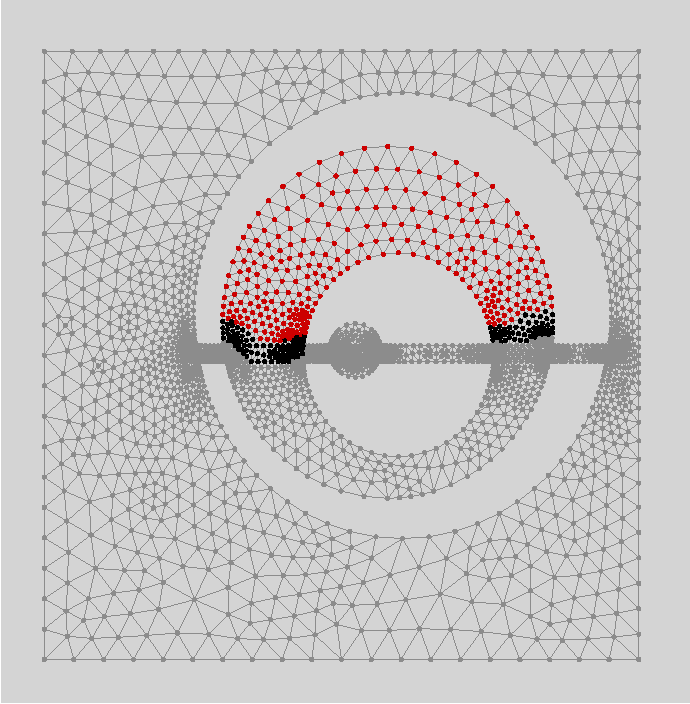
\includegraphics[width=\linewidth]{hole-mesh-core-1-eps-converted-to}
& 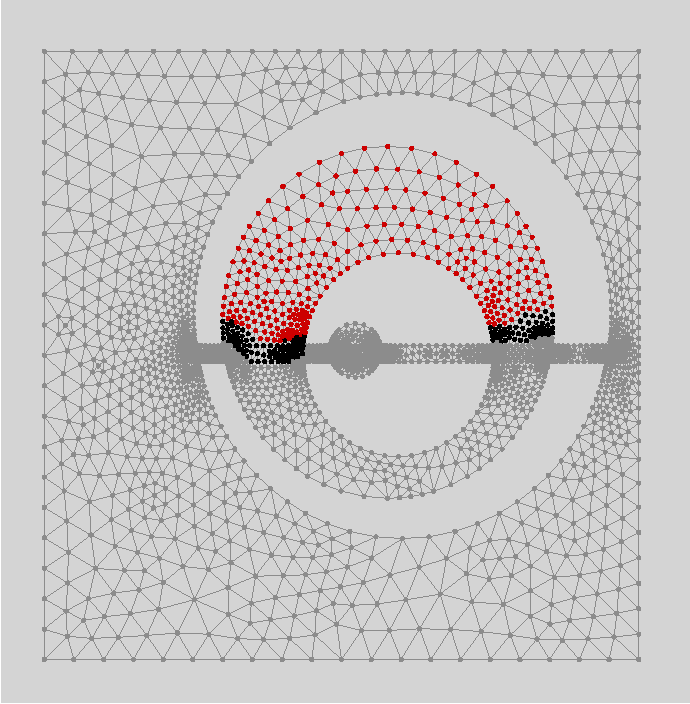
\includegraphics[width=\linewidth]{hole-mesh-core-1-eps-converted-to}
\\
A combined cluster \newline
(red = home vertices)
& ... and another
\\
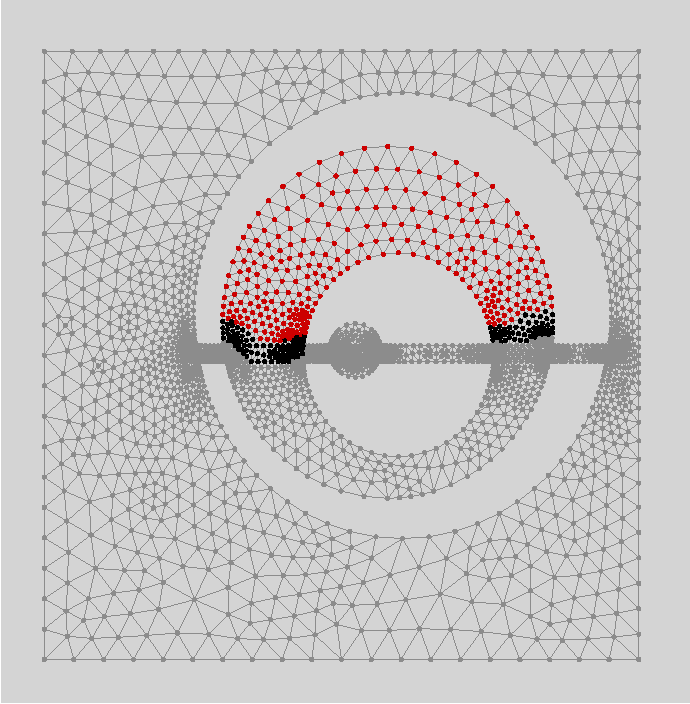
\includegraphics[width=\linewidth]{hole-mesh-core-1-eps-converted-to}
& 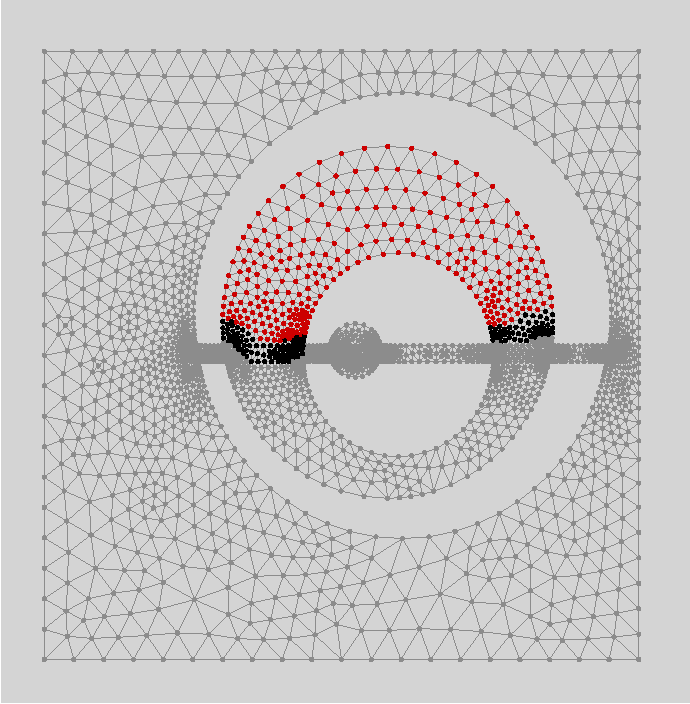
\includegraphics[width=\linewidth]{hole-mesh-core-1-eps-converted-to}
\\
Overall best containment
(white=best)
& Vertex overlap \newline
(gray=1, black=2, red=2)
\\
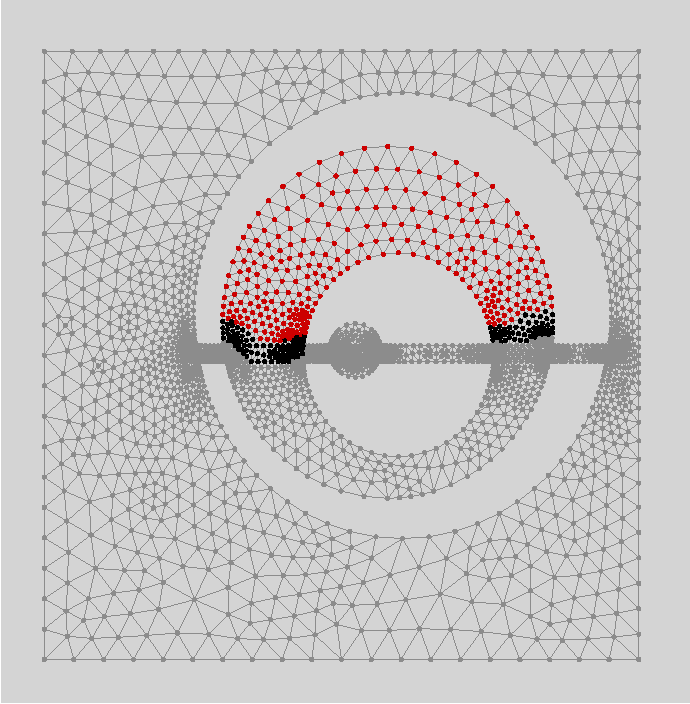
\includegraphics[width=\linewidth]{hole-mesh-core-1-eps-converted-to}
& 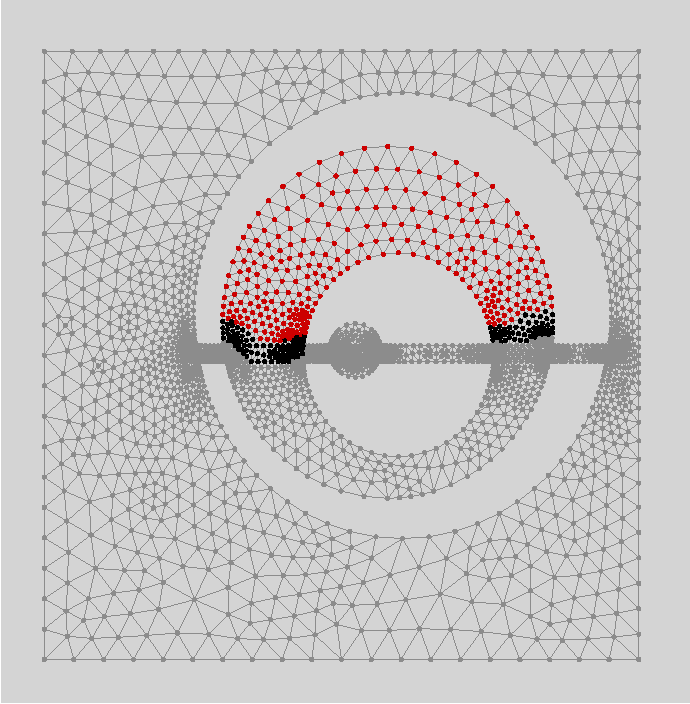
\includegraphics[width=\linewidth]{hole-mesh-core-1-eps-converted-to}
\end{tabular}

\end{beamercolorbox}
}
\end{center}



\end{block}



\postercolumn[t]{0.25\textwidth}
\begin{block}{5. Data}
 \RaggedRight
 
We empirically study this idea on 10 public graphs.  
\begin{center}
\footnotesize
%\rowcolors{1}{rowshade1}{rowshade2}
\begin{tabularx}{0.9\linewidth}{rXXXX}
  \rowcolor{background} \rule{0pt}{2.5ex} 
  Graph & $|V|$ & $|E|$ & $\max \deg$ & $|E|/|V|$ \\
  \rowcolor{neutralshade} \dataname{onera} &    85567 &   419201   &        5 &    4.9         
\\ \rowcolor{neutralshade} \dataname{usroads} &   126146 &   323900   &        7 &    2.6           
\\ \rowcolor{neutralshade} \dataname{annulus} &   500000 &  2999258   &       19 &    6.0       
\\ \rowcolor{neutralshade}  \dataname{email-Enron} &    33696 &   361622   &     1383 &   10.7          
\\ \rowcolor{neutralshade}  \dataname{soc-Slashdot} &    77360 &  1015667   &     2540 &   13.1          
\\ \rowcolor{neutralshade} \dataname{ dico} &   111982 &  2750576   &    68191 &   24.6          
\\ \rowcolor{neutralshade}   \dataname{lcsh} &   144791 &   394186   &     1025 &    2.7          
\\ \rowcolor{neutralshade}  \dataname{web-Google} &   855802 &  8582704   &     6332 &   10.0          
\\ \rowcolor{neutralshade}   \dataname{as-skitter} &  1694616 & 22188418   &    35455 &   13.1          
\\ \rowcolor{neutralshade}    \dataname{cit-Patents} &  3764117 & 33023481   &      793 &    8.8
 \end{tabularx}
\end{center}


\end{block}

\begin{block}{6. Results}
\RaggedRight

We present two types of results: (i)  an
 estimated swapping probability $\rho_{\infty}$; 
 and (ii) the communication volume of a parallel PageRank
solution (link-following $\alpha=0.85$) using an 
additive Schwarz method.  The volume ratio is the amount of
extra storage for the overlap (2 means we store the graph twice).
Below, as the ratio increases, the swapping
probability and PageRank communication volume decreases.
% \begin{center}
% \fcolorbox{neutralshade}{neutralshade}{
%   \begin{beamercolorbox}[sep=0.25\em,wd=0.6\linewidth]{mybox}  
%    \centering
%    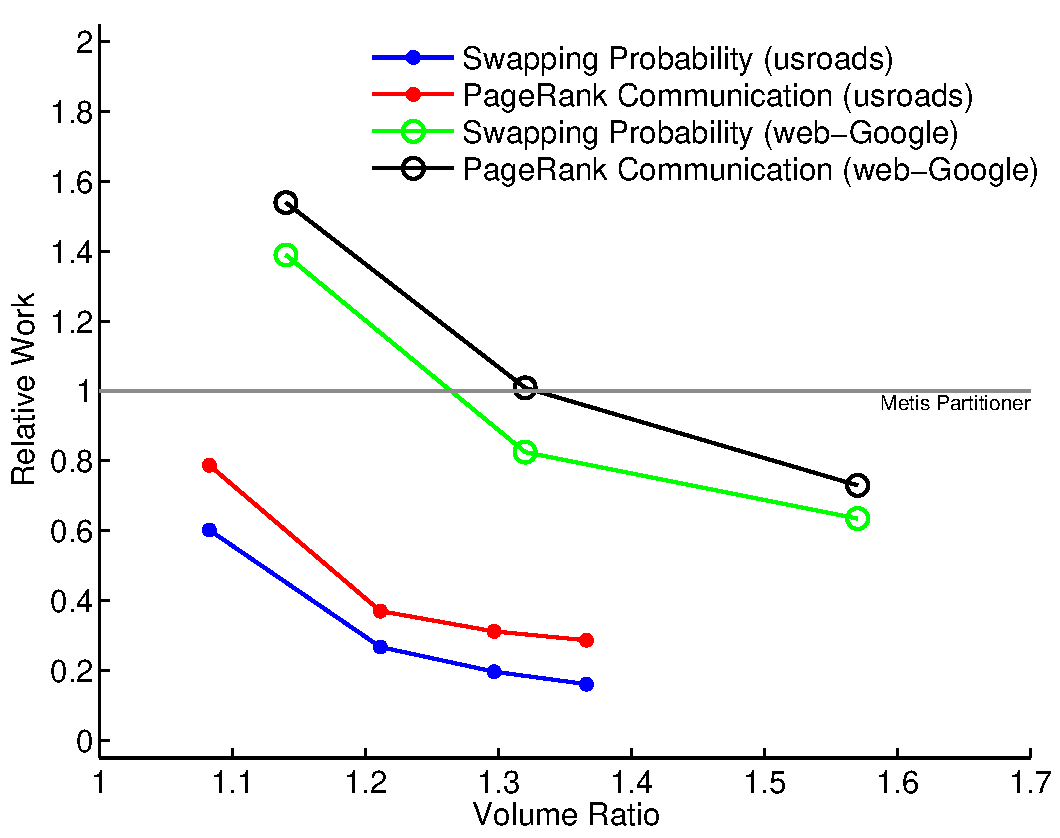
\includegraphics[width=0.6\linewidth]{overlap-benefit-combined-eps-converted-to}
%   \end{beamercolorbox}
% }
% \end{center}

\begin{center}
\footnotesize
\fcolorbox{neutralshade}{neutralshade}{
\begin{beamercolorbox}[sep=0.25em,wd=\linewidth]{mybox}
\centering%
\begin{tabularx}{\linewidth}{Xp{13cm}Xp{13cm}X}
& Two graphs, in detail
& & All graphs, multiple experiments.
\\
  & 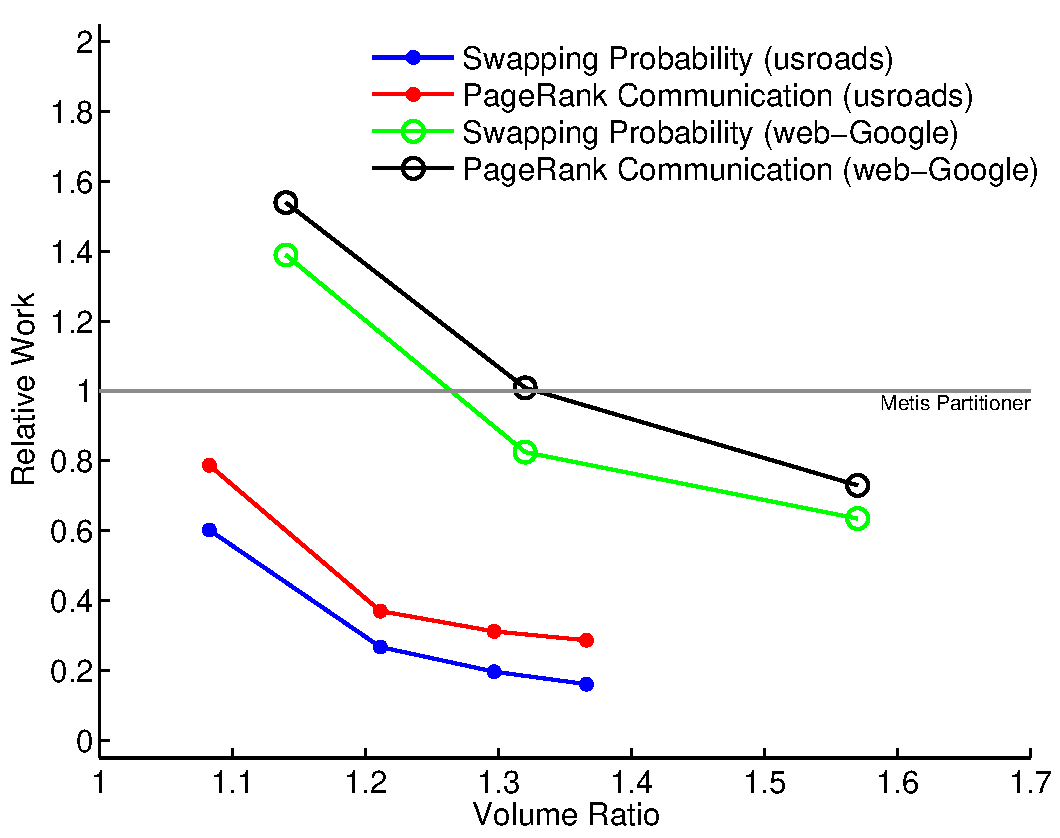
\includegraphics[width=\linewidth]{overlap-benefit-combined-eps-converted-to}
  & & 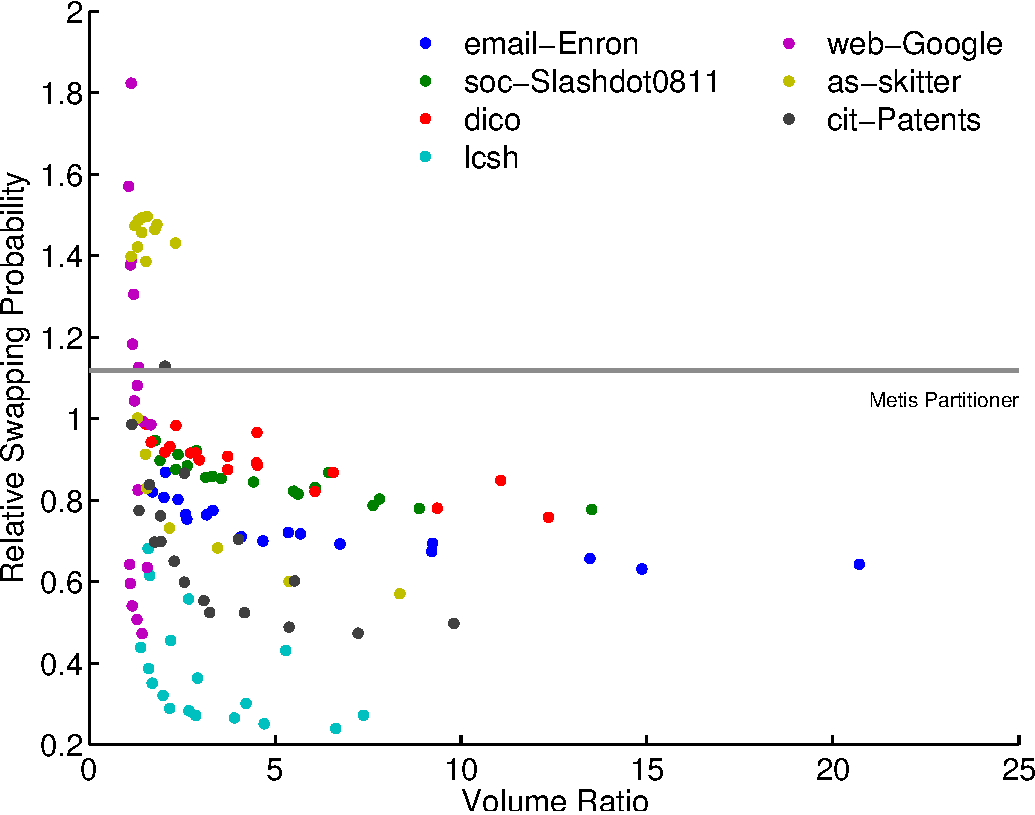
\includegraphics[width=\linewidth]{swapping-probability-indiv-poster-eps-converted-to}
  & 
\end{tabularx}
\end{beamercolorbox}
}
\end{center}



The communication ratio of our best
result for the PageRank communication volume compared to 
{\small \textsc{METIS}} or {\small \textsc{GRACLUS}} shows
that the method works for 6 of them (perf.~ratio $< 1$).
The 0 communication result is not a bug.
\begin{center}
\footnotesize
%\rowcolors{1}{rowshade1}{rowshade2}
\begin{tabularx}{0.9\linewidth}{lVVVV}
\rowcolor{background} \rule{0pt}{2.5ex} Graph & Comm. of Partition  & Comm. of Overlap  & Perf. Ratio & Vol. Ratio \\
\rowcolor{neutralshade}  \dataname{onera}  & 18654  & 48  & 0.003 & 2.82   \\
\rowcolor{neutralshade} \dataname{usroads}  & 3256 & 0 & 0.000 & 1.49   \\
\rowcolor{neutralshade} \dataname{annulus}  & 12074  & 2 & 0.000 & 0.01   \\
\rowcolor{neutralshade} \dataname{email-Enron}  & 194536* & 235316  & 1.210 & 1.7  \\
\rowcolor{neutralshade} \dataname{soc-Slashdot} & 875435* & ${1.3 \times 10^6}$ & 1.480 & 1.78   \\
\rowcolor{neutralshade} \dataname{dico} & $1.5 \times 10^{6}$*   & ${2.0 \times 10^6}$ & 1.320 & 1.53\\
\rowcolor{neutralshade} \dataname{lcsh} & 73000*  & 48777 & 0.668 & 2.17   \\
\rowcolor{neutralshade} \dataname{web-Google} & 201159*  & 167609  & 0.833 & 1.57  \\
\rowcolor{neutralshade} \dataname{as-skitter} & $2.4 \times 10^{6}$ & ${3.9 \times 10^6}$ & 1.645 & 1.93   \\
\rowcolor{neutralshade} \dataname{cit-Patents}  & $8.7 \times 10^{6}$ & ${7.3 \times 10^6}$ & 0.845 & 1.34 \\
 \end{tabularx}
\end{center}

Finally, we evaluate our heuristic.
\vspace{-1.5ex}

\begin{center}
\footnotesize
\fcolorbox{neutralshade}{neutralshade}{
\begin{beamercolorbox}[sep=0.25em,wd=\linewidth]{mybox}
\centering%
\begin{tabular}{@{\hfill}p{7.5cm}@{\hfill}p{7.5cm}@{\hfill}p{7.5cm}@{\hfill}}
\multicolumn{3}{p{22.5cm}}{%
  At left, the cluster combine procedure reduces $10^6$ clusters to around $10^2$.
  Middle, combining clusters can decrease the volume ratio from 10 to around 1.
  At right, the mean conductance tends to decrease after combining clusters.
  }
\\
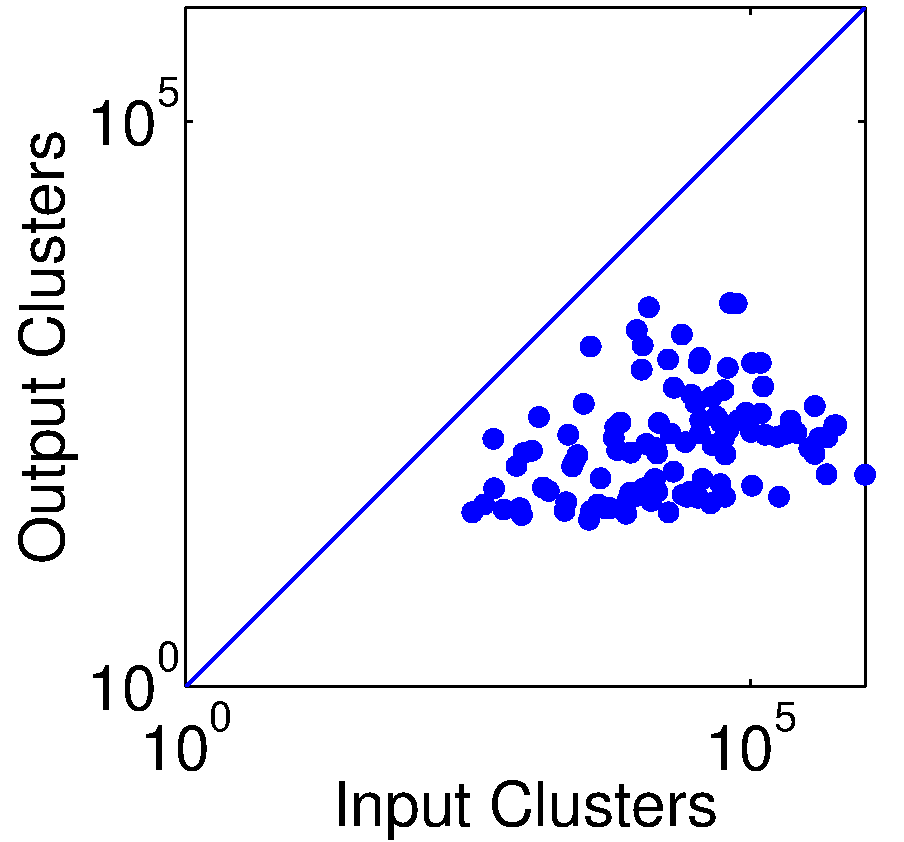
\includegraphics[width=\linewidth]{combine-cluster-change-eps-converted-to}
 & 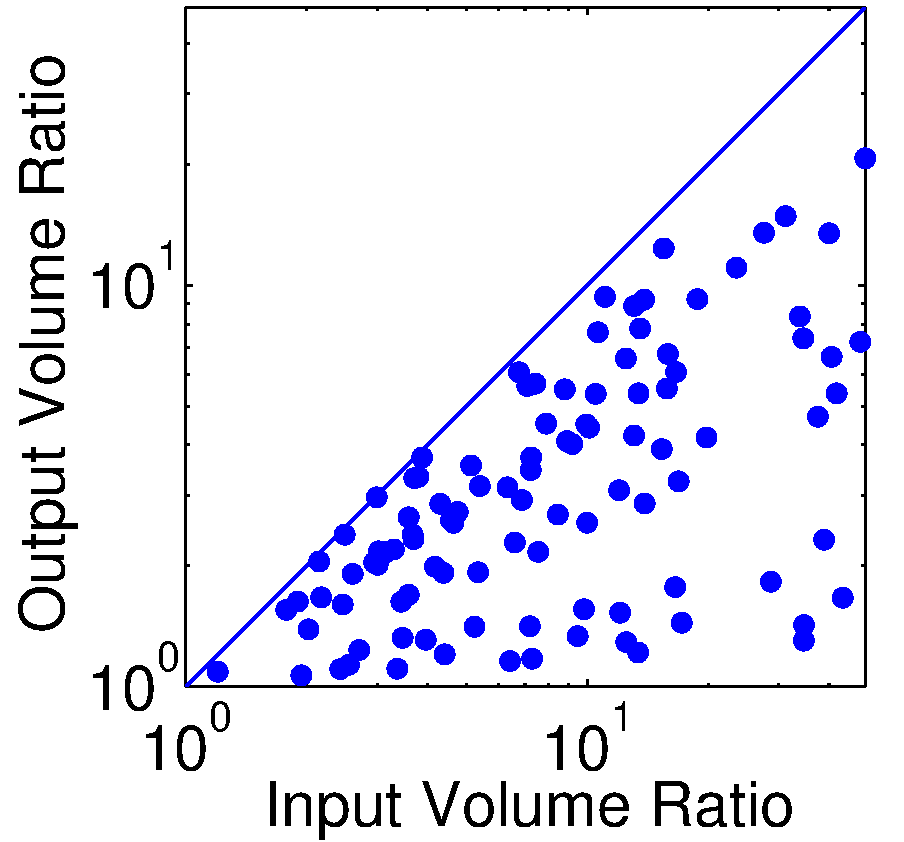
\includegraphics[width=\linewidth]{combine-volume-reduction-eps-converted-to}
 & 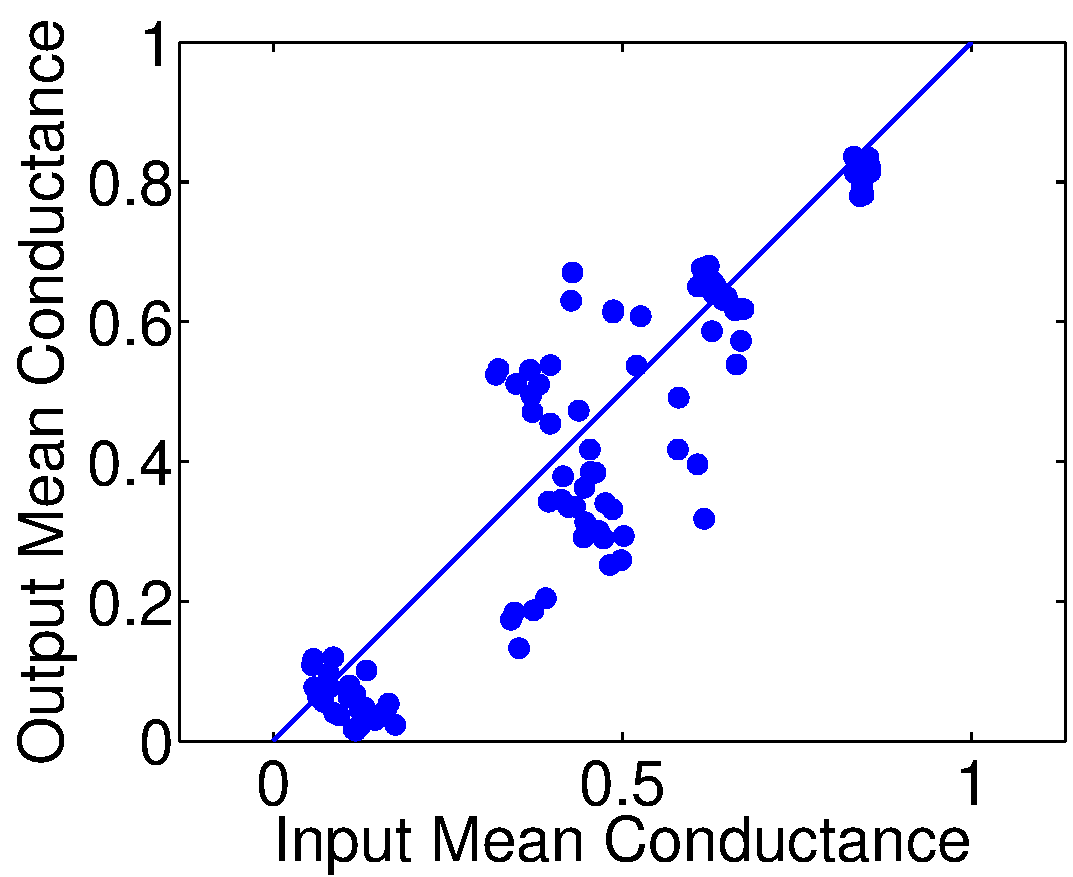
\includegraphics[width=\linewidth]{combine-conductance-change-eps-converted-to}
% \multicolumn{3}{p{22.5cm}}{%
%   From left to right, a sample power law graph,
%   a sample graph with the exact matches, and
%   the totally random matches.  Again, the bright
%   red edges are random perturbations.}
\end{tabular}
\end{beamercolorbox}
}
\end{center}

\end{block}

\end{columns}

%% A beamerposter only has a single frame, end the global frame
\end{frame}
\end{document}
